Hiring effective candidates is one of the key challenges faced by any organization.
There are two possibly conflicting optimization issues that a hiring committee faces when considering who to hire: 
(i) the value added to the organization in terms of the candidate's raw skills and competencies, and 
(ii) how well the candidate can collaborate with the existing members of the organization.
The first consideration depends on the complementarity between the candidate's skills and the tasks that the organization aims to complete. 
This is called \textit{coverage} in the team formation literature.
The second consideration is commonly known as the \textit{communication cost}.

In their seminal paper, Lappas et al. \cite{lappas2009finding} first introduced the \textit{team formation} problem, where they modelled a the organization as an undirected graph and a team as an induced subgraph of the organization.

They proposed two graph distance-based measures of communication cost, namely the diameter and minimum spanning tree of the graph. 
They showed that the team formation problem is NP-complete for both types of communication costs. 
Subsequent works \cite{sozio2010community, kargar2011discovering, anagnostopoulos2010power, rangapuram2013towards} explored more realistic formulations of the team  formation problem. They study different cost functions and objectives that model the real world requirements more closely.
In \cite{bhowmik2014submodularity}, a submodular variant of the team formation problem is proposed, enabling an approximation guarantee for a simulated annealing algorithm.

Our work distinguishes itself by studying the problem of team formation from a organization's point of view. In a typical organization the exact set of tasks is not known beforehand. The tasks vary depending on the progress the organization makes in different fronts. However, the organization does need to make decisions regarding the employees, such as whom to hire or fire based on a possible task assignment in an expected sense. Moreover  

Our work distinguishes itself from these previous studies in that we consider the problem of adding a new member to an already-existing team, whereas the other works concern themselves with forming teams from scratch.
>>>>>>> fd72645f9785138025d541e9992cc4f67c10f95f
Our problem can thus be better viewed as a \textit{hiring problem}. Moreover, we consider the scenario where the set of tasks to complete is not known with certainty.
In \cite{anagnostopoulos2012online}, it is assumed that tasks arrive in an online manner, and teams are formed on the fly.
In our problem formulation, we assume that the organization also forms teams online for an infinite stream of tasks drawn from a known probability distribution.
We want to hire candidates so as to maximize the resulting team's ability to complete tasks drawn from this distribution.

To understand this better, refer to Figure \ref{fig:hpo}.
Our problem has three inputs: an existing organization, a pool of candidates, and a task distribution. 
Our goal is to find a set of candidates from the pool that maximizes the expected coverage while adding minimum communication overhead, and does not exceed a hiring budget. 
\begin{figure}
\centering
\begin{small}
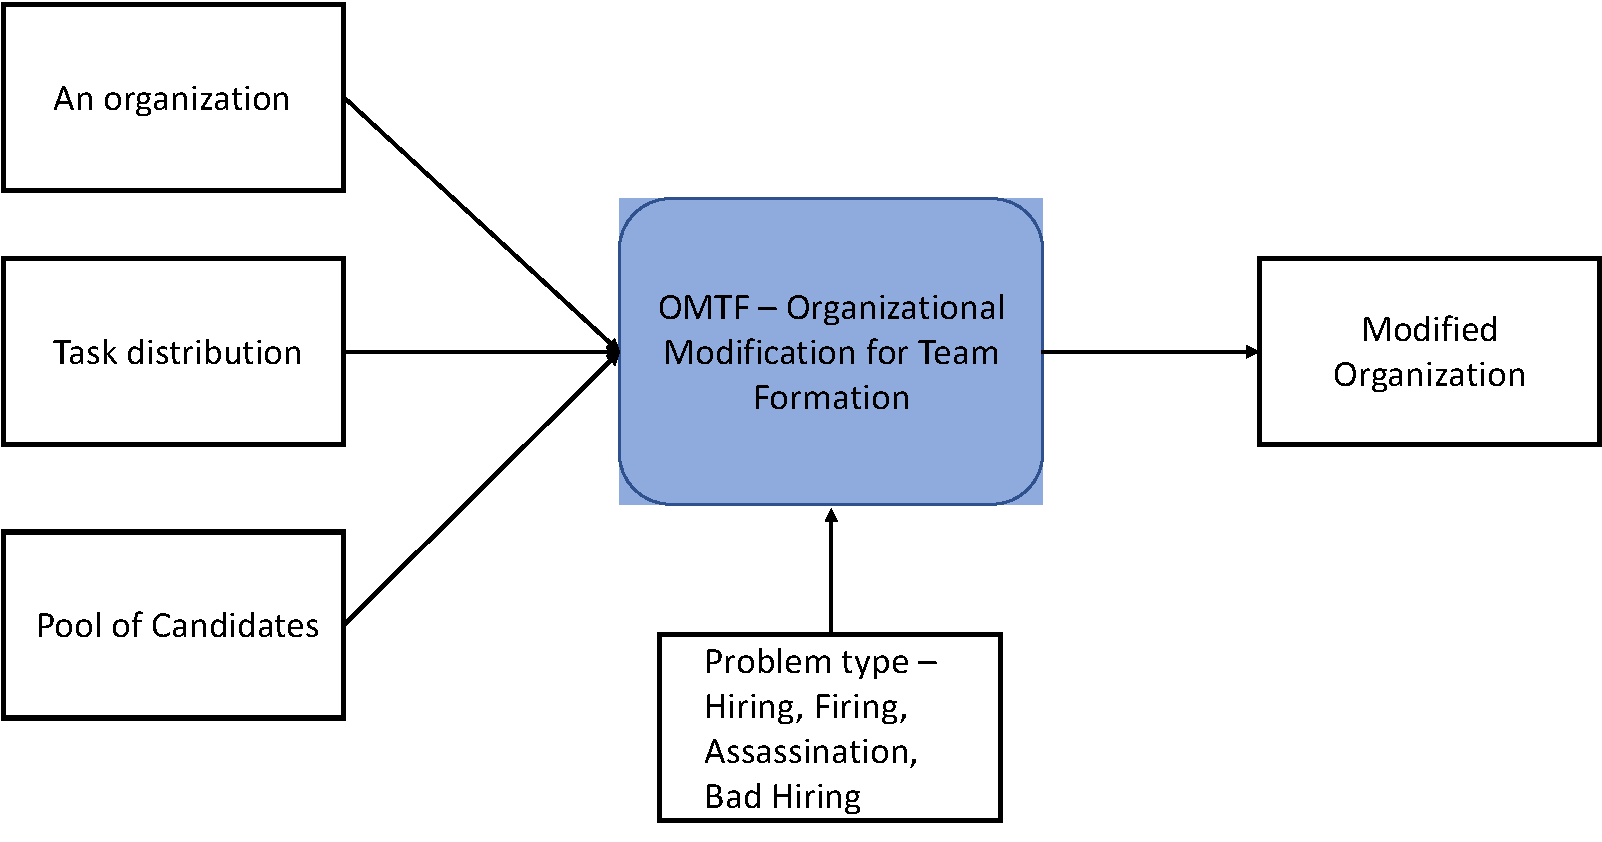
\includegraphics[width=.25\textwidth]{figs/pdf/illustration.pdf}
\caption{Hiring problem overview}
\label{fig:hpo}
\end{small}
\end{figure} 

In this paper, we show that the hiring problem is NP-hard.
However, we provide two realistic communication and coverage functions such that both are submodular.
Thus, to summarize, our contributions are the following:

\begin{enumerate}
\item We formulate the novel \textit{hiring problem}, which draws its inspiration from the team formation literature.

\item We show that the problem is NP-hard. 

%\item By leveraging the work of \cite{bai2016algorithms}, we design a greedy algorithm that preserves a $1 - \frac{1}{e}$ approximation ratio.

\item Through extensive experiments on real world datasets, we empirically show the superiority of our approach over existing baselines. 

\end{enumerate}